\section{Verschiedene Versionen der Anzeige}
\setauthor{Oliver Sugic}
Für die graphische Oberfläche wurden verschiedene Ideen und Konzepte ausprobiert, um die Benutzbarkeit für die Lernenden und Lehrenden zu optimieren.
Im Laufe des Kapitels wird erläutert, welche Versionen der Anzeige es gab und welche Versionen sich als sinnvoll erwiesen haben.

\subsection{Version 1: Visualisierung mit Karten}
\setauthor{Oliver Sugic}
Am Anfang wurden Überlegungen angestellt, wie man die Lernenden als auch die Lehrenden am besten in nicht vertrautes Gebiet führen kann.
Da die meisten Person mit Kartenservices, wie beispielsweise Google Maps oder ähnlichen Dienstleistungen, vertraut sind, wurde eine Karte implementiert.
Es gibt viele verschiedene Anbieter von Kartenservices, die in Betracht gezogen wurde. 
Da Google Maps eines der bekanntesten Anbieter, wurde auf die Google Maps Api gesetzt. 
Doch im Laufe der Recherche ist klar geworden, dass die Google Maps Api nicht die beste Lösung für dieses Projekt ist  aus folgenden Gründen
\begin{itemize}
    \item Die Google Maps Api läuft über die Google Cloud und ist daher kostenpflichtig
    \item Google Maps Api ist nicht open-source
    \item Google Maps Api ist nicht einfach zu anzupassen an die Bedürfnisse des Projektes 
\end{itemize}
%\cite{}

\cite{Agafonkin} Auf der Suche nach weiteren Alternativen, verwies mich Herr Pavelescu auf die Open-Source Kartenlösung Leaflet.
Leaflet ist eine JavaScript Libary, die es ermöglicht, Karten in Webanwendungen zu integrieren. 


\pagebreak

\begin{lstlisting}[numbers=left,language=HTML,caption={Implementierung einer Karte mit Leaflet},label={lst:leafletmap}]{}
    <style>
    #map { height: 1000px; }
    </style>
    </head>
    <body>
     <link rel="stylesheet" href="https://unpkg.com/leaflet@1.9.3/dist/leaflet.css"
         integrity="sha256-kLaT2GOSpHechhsozzB+flnD+zUyjE2LlfWPgU04xyI="
         crossorigin=""/>
    
     <script src="https://unpkg.com/leaflet@1.9.3/dist/leaflet.js"
         integrity="sha256-WBkoXOwTeyKclOHuWtc+i2uENFpDZ9YPdf5Hf+D7ewM="
         crossorigin=""></script>
    
     <div id="map"></div>
      <script>
    var map = L.map('map').setView([48.2684159, 14.2517532], 20);
    L.tileLayer('https://tile.openstreetmap.org/{z}/{x}/{y}.png', {
        maxZoom: 19,
        attribution: '&copy; <a href="http://www.openstreetmap.org/copyright">OpenStreetMap</a>'
    }).addTo(map);
    </script> 
\end{lstlisting}

\begin{figure}[h]
\centering
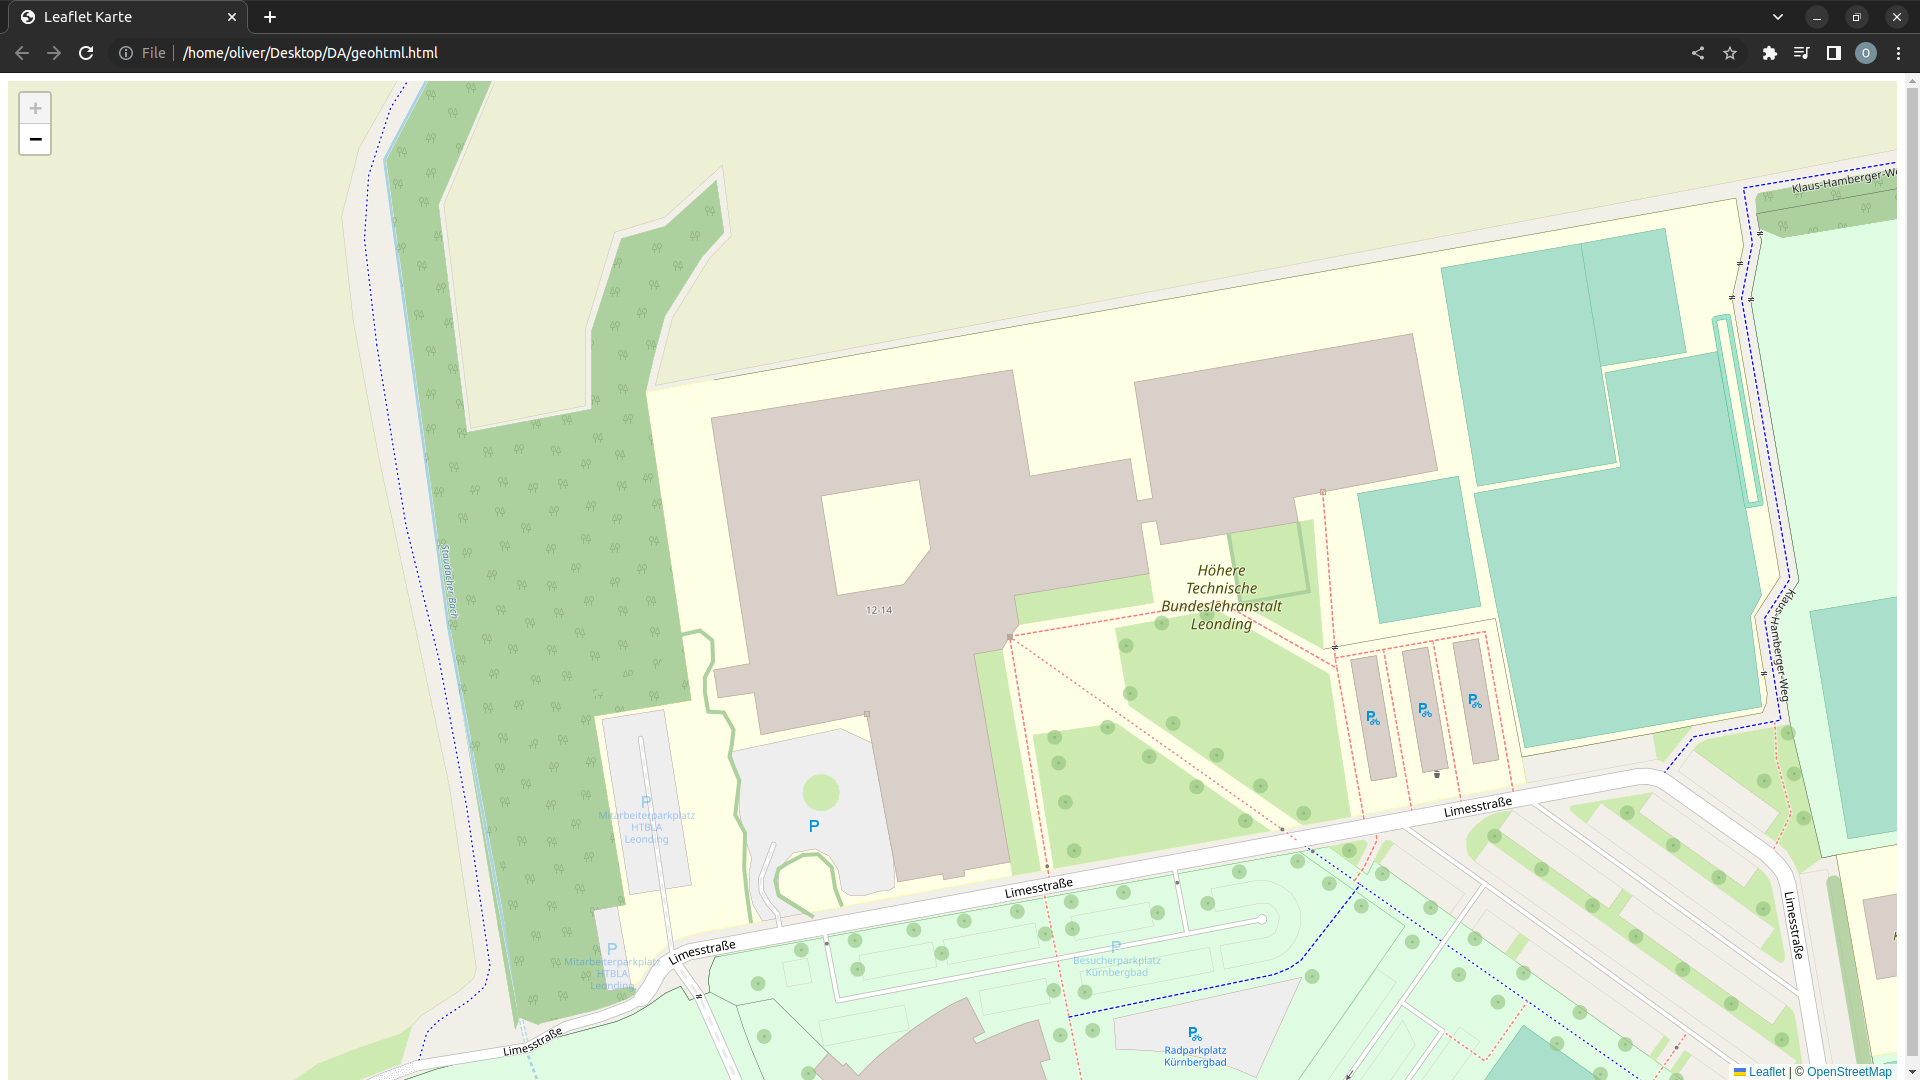
\includegraphics[scale=0.2]{pics/leafletmap.png}
\caption{Ergebnis der Implementierung mit Leaflet}
\end{figure}


\subsection{Version 2: Leaflet Karte mit Routing}
\setauthor{Oliver Sugic}
Nach dem ersten Prototypen mit Leaflet, wurde die Idee weiter verfolgt, um die Benutzerfreundlichkeit für die Teilnehmenden zu verbessern. Eine Route vom eigenen Standort zur nächsten Aktivität wurde implementiert. Um die Routen anzeigen zu können, wurde die Leaflet Routing Machine verwendet. 
Hierfür wird das Plugin Leaflet Routing Machine verwendet, das ebenfalls vom Leaflet zur Verfügung gestellt wird. Mit dieser Erweiterung Können Routen zwischen zwei Punkten auf der Karte berechnet werden und angezeigt werden. Ebenfalls können die Wegpunte einfach geändert werden.

\begin{lstlisting}[numbers=left,language=HTML,caption={Implementierung einer Karte mit Leaflet Routing Engine},label={lst:leafletmap}]
    <head>
    <title>Leaflet Karte</title>
    <style>
        #map {
            height: 1500px;
        }
    </style>
</head>

<body>
    <link rel="stylesheet" href="https://unpkg.com/leaflet@1.9.3/dist/leaflet.css"
        integrity="sha256-kLaT2GOSpHechhsozzB+flnD+zUyjE2LlfWPgU04xyI=" crossorigin="" />

    <script src="https://unpkg.com/leaflet@1.9.3/dist/leaflet.js"
        integrity="sha256-WBkoXOwTeyKclOHuWtc+i2uENFpDZ9YPdf5Hf+D7ewM=" crossorigin="">
        </script>
    <link rel="stylesheet" href="https://unpkg.com/leaflet@1.2.0/dist/leaflet.css" />
    <link rel="stylesheet" href="https://unpkg.com/leaflet-routing-machine@latest/dist/leaflet-routing-machine.css" />
    <script src="https://unpkg.com/leaflet@1.2.0/dist/leaflet.js"></script>
    <script src="https://unpkg.com/leaflet-routing-machine@latest/dist/leaflet-routing-machine.js"></script>

    <div id="map"></div>
    <script>
        var map = L.map('map').setView([48.2684159, 14.2517532], 15);
        L.tileLayer('https://tile.openstreetmap.org/{z}/{x}/{y}.png', {
            maxZoom: 19,
            attribution: '&copy; <a href="http://www.openstreetmap.org/copyright">OpenStreetMap</a>'
        }).addTo(map);
        L.Routing.control({
            waypoints: [
                L.latLng(48.2684159, 14.2517532),
                L.latLng(48.2627373, 14.2589871)
            ]
        }).addTo(map);
    </script>
\end{lstlisting}
\begin{figure}[h]
    \centering
    \includegraphics[scale=0.2]{pics/Leaflet_Routing.png}
    \caption{Ergebnis der Implementierung mit Leaflet Routing Machine}
\end{figure}

Allerding traten bei der Implementierung Probleme auf. Das Plugin konnte allerdings nicht die Route darstellen, was auf einen Fehler in der Implementierung zurückzuführen war.

\subsection{Version 3: Angular Geoloaction API}
\setauthor{Oliver Sugic}
Nach dem Scheitern der Implementierung mit der Leaflet Routing Machine, wurde eine neues Design entworfen, um die Benutzerfreundlichkeit zu verbessern.
Nach vielen Überlegung wurde ein Wireframe designed \ref{lst:Wireframe}, welches sowohl für mobile Endgeräte geeignet ist, aber auch überschaulich für die nutzenden Personen ist.

\begin{figure}[h]
    \centering
    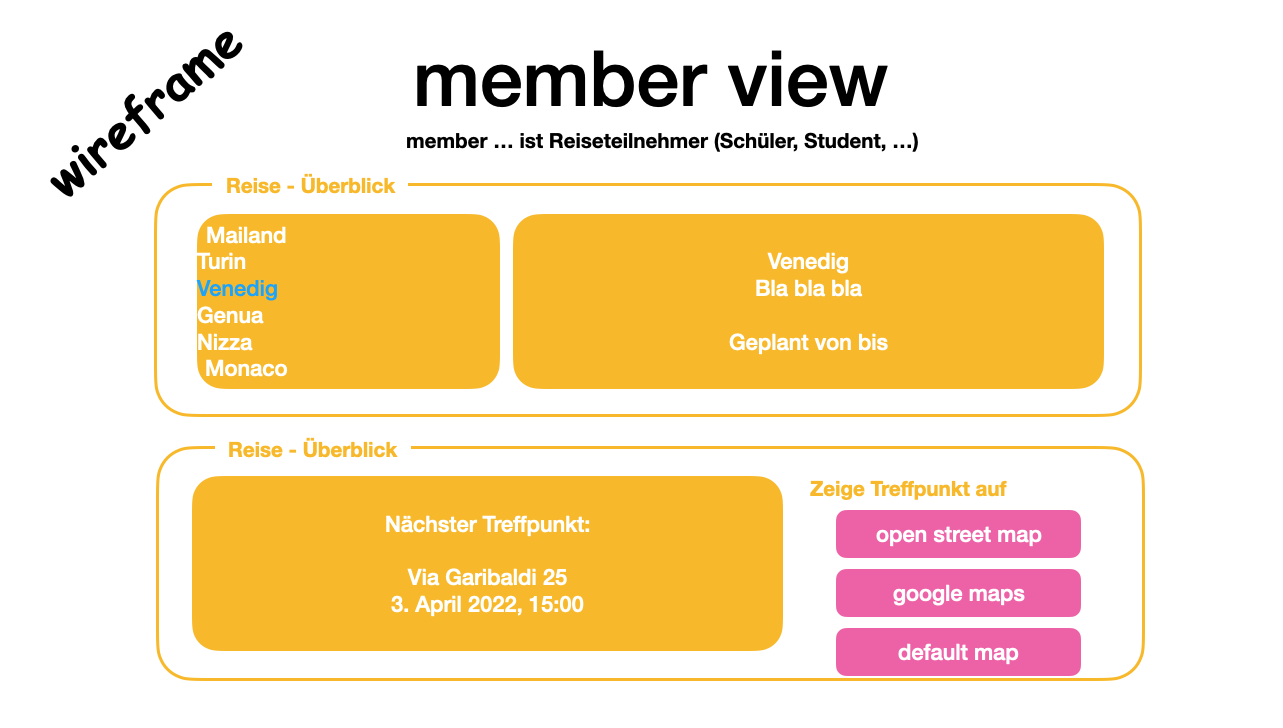
\includegraphics[scale=0.2]{pics/Wireframe.png}
    \caption{Endgültige Version }
    \label{lst:Wireframe}
\end{figure}

Der Nutzer soll in einen groben Überblick haben, welche Städte er besuchen wird. Durch eine kurze Beschreibung der Aktivität solle der Reisende einen kurzen Einblick haben, was Ihn erwarten wird. In der unteren Hälfte des Bildschrim erhält man genauere Informationen über den Treffpunkt, außerdem ist es möglich sich auf der Karte die Route anzeigen zu lassen. Es ist möglich, sich auf der standartmäßigen Karte des Endgeräts, über Google Maps oder über die OpenStreetMap zu navigieren. Der Nutzende kann für sich entscheiden, welche Karte Ihm am besten gefällt oder welche Karte Ihm am meisten vertraut ist. 

\section{Aktuelle Komponenten}
\setauthor{Oliver Sugic}
Derzeit besteht die Anwendung aus drei Komponenten. In diesem Kaptiel werden der Aufbau und und Zusammenhäbge der einzelen Komponenten erläutert.  


\subsection{Angular Frontend}
\setauthor{Oliver Sugic}

Der schwierigste Teil der Arbeit liegt in darin, eine Benutzeroberfläche zu erstellen, die einfach zu bedienen aber auch ansprechend für den Benutzer ist.


\subsection{Quarkus Backend }
\setauthor{Oliver Sugic}

\subsection{Keycloak}
\setauthor{Oliver Sugic}

\subsection{Mögliche zukünftige Erweiterungen}
\setauthor{Oliver Sugic}


